\documentclass[10pt]{beamer}
\usetheme{Frankfurt}
\usepackage[utf8]{inputenc}
\usepackage[spanish,es-tabla]{babel}
\usepackage{amsmath}
\usepackage{amsfonts}
\usepackage{amssymb}
\usepackage{graphicx}
\graphicspath{{imagenes/}}									% Ruta de las imagenes, solo escribir nombre de la imagen
\author{Ciro Fabián Bermúdez Márquez}
\title{Optimización de dimensión oscilador utilizando }
%\setbeamercovered{transparent} 
%\setbeamertemplate{navigation symbols}{} 
%\logo{} 
\institute{Benemérita Universidad Autónoma de Puebla} \date{6 de Febrero de 2020} 
%\subject{}

%-------------------------------------------------------------------------------
%                        Paquetes para hipervinculos                           %
%-------------------------------------------------------------------------------


%---------------------------------------------------------------------
%                      Paquetes adicionales                          %
%---------------------------------------------------------------------
\decimalpoint
\usepackage{xcolor}
\usepackage{ragged2e}
\usepackage{etoolbox}

\usepackage{comment}											% Comentarios largos
\usepackage{pdfpages}											% Incluir portada echa en Inkscape
\usepackage{setspace}											% Interlineado
\usepackage{makecell}											% Para tablas
\usepackage{xcolor}												% Colores en tablas
\usepackage{colortbl}
\usepackage{array}												% Necesario para algunas tablas
\usepackage[inline]{enumitem}									% Personalizar itemize
\usepackage{multicol}											% Item 2 columns											% Necesario para algunas tablas
\usepackage{subcaption}											% Subfiguras
%-------------------------------------------------------------------------------
%                            Comandos matematicos                              %
%-------------------------------------------------------------------------------
\usepackage{steinmetz}											% Para representar fasores
\usepackage{bm}													% Bold math  \bm command
\newcommand{\binomb}[2]{\genfrac{[}{]}{0pt}{}{#1}{#2}}


\apptocmd{\frame}{}{\justifying}{} % Allow optional arguments after frame.

\setbeamertemplate{footline}
{
  \leavevmode%
  \hbox{%
  \begin{beamercolorbox}[wd=.333333\paperwidth,ht=2.5ex,dp=1ex,center]{author in head/foot}%
    \usebeamerfont{author in head/foot}Ciro Fabián Bermúdez Márquez
  \end{beamercolorbox}%
  \begin{beamercolorbox}[wd=.333333\paperwidth,ht=2.5ex,dp=1ex,center]{title in head/foot}%
    \usebeamerfont{title in head/foot}Benemérita Universidad Autónoma de Puebla
  \end{beamercolorbox}%
  \begin{beamercolorbox}[wd=.333333\paperwidth,ht=2.5ex,dp=1ex,right]{date in head/foot}%
    \usebeamerfont{date in head/foot}Facultad de Ciencias de la Electrónica\hspace*{2em}
    \insertframenumber{} / \inserttotalframenumber\hspace*{2ex} 
  \end{beamercolorbox}}%
  \vskip0pt%
}


%\usefonttheme{serif}
\usefonttheme[onlymath]{serif}



\setbeamertemplate{caption}[numbered]
\theoremstyle{definition}
	\newtheorem{defn}{Definición}
	\newtheorem{exmp}{Ejemplo}
	\newtheorem{law}{Ley}
	
	
%-------------------------------------------------------------------------------
%                            Libreria de codigos                               %
%-------------------------------------------------------------------------------
% Paquetes necesarios
\usepackage{listings}
\usepackage{xcolor}

% Tipos de letra personalizadas
\def\lstbasicfont{\fontfamily{pcr}\selectfont\scriptsize}
\def\vhdlbasicfont{\fontfamily{cmtt}\selectfont\scriptsize}

% Colores personalizados
\definecolor{codegreen}{rgb}{0,0.6,0}
\definecolor{codepurple}{rgb}{0.58,0,0.82}

\definecolor{codegray}{rgb}{0.5,0.5,0.5}
\definecolor{backcolour}{rgb}{0.95,0.95,0.92}
\definecolor{codeorange}{RGB}{254, 100, 35}

% Deficion de lenguajes perzonalizados

% Definicion de lenguaje MATLAB
\lstdefinelanguage{matlabfloz}{%
  alsoletter={...},%
  morekeywords={%                             % keywords
		break,case,catch,classdef,continue,else,
		elseif,end,for,function,global,if,
		otherwise,parfor,persistent,
		return,spmd,switch,try,while,...},        % Use the matlab "iskeyword" command to get those
  comment=[l]\%,                              % comments
  morecomment=[l]...,                         % comments
  morecomment=[s]{\%\{}{\%\}},                % block comments
  morestring=[m]'                             % strings 
}[keywords,comments,strings]%

% Estilos MATLAB
\lstdefinestyle{MATLAB}{
	frame=single,
	rulecolor=\color{black},
	framexleftmargin=4mm,
	xleftmargin=2mm,
	language=matlabfloz,
  commentstyle=\color{codegreen},
  keywordstyle=\color{blue}, %magenta
  numberstyle=\tiny\color{black},
  stringstyle=\color{codepurple},
  basicstyle=\lstbasicfont\tiny,
  breakatwhitespace=false,         
  breaklines=true,                 
  captionpos=b,                    
  keepspaces=true,                 
  numbers=left,                    
  numbersep=5pt,                  
  showspaces=false,                
  showstringspaces=false,
  showtabs=false,                  
  tabsize=2    
}

% Estilos MATLAB en codigo
\lstdefinestyle{MATLAB_preview}{
%	frame=single,
%	rulecolor=\color{black},
%	framexleftmargin=4mm,
%	xleftmargin=2mm,
	language=matlabfloz,
    commentstyle=\color{codegreen},
    keywordstyle=\color{blue}, %magenta
%    numberstyle=\tiny\color{black},
    stringstyle=\color{codepurple},
    basicstyle=\lstbasicfont\small,
    breakatwhitespace=false,         
    breaklines=true,                 
    captionpos=b,                    
    keepspaces=true,                 
%    numbers=left,                    
%    numbersep=5pt,                  
    showspaces=false,                
    showstringspaces=false,
    showtabs=false,                  
    tabsize=2    
}

\renewcommand{\lstlistingname}{Código}% Listing -> Algorithm
\renewcommand{\lstlistlistingname}{Lista de códigos}% 

\begin{document}
%%----------------------------------------------------------------------------------
%%----------------------------------------------------------------------------------
	\begin{frame}[plain]
	
		%\begin{center}
		%	\textbf{Facultad de Ciencias de La Electrónica}
		%\end{center}
		
		\begin{center}
			\textcolor{blue}{Instituto Nacional de Astrofísica, Óptica y Electrónica.}
		\end{center}
		
		\begin{figure}[hbtp]
			\centering
			
\includegraphics[width = 2.5cm]{logoinaoe.png} 
		\end{figure}
		
		\begin{center}
			\textbf{Maestría en Ciencias en la Especialidad de Electrónica}
		\end{center}
						
		\begin{center}
			\begin{Large}
			\textcolor{blue}{Optimización de dimensión KY del oscilador caótico SNLF  utilizando evolución diferencial}
			\end{Large}
		\end{center}
		
		\begin{center}
			\textbf{Ciro Fabián Bermúdez Márquez }
		\end{center}
		
		\begin{center}
			\textbf{Asesor:} Dr. Esteban Tlelo Cuatle
		\end{center}
	\end{frame}
%%----------------------------------------------------------------------------------
%%----------------------------------------------------------------------------------
	\begin{frame}
		\tableofcontents
	\end{frame}
%%----------------------------------------------------------------------------------
%%----------------------------------------------------------------------------------
	\section{Introducción}
	\begin{frame}
	\frametitle{Introducción}
		\begin{block}{¿Qué es el caos?}
		\justifying
			El caos se refiere a un tipo de comportamiento dinámico complejo que posee algunas características muy especiales:
			\begin{itemize}
				\item Se describe mediante un conjunto de ecuaciones diferenciales ordinarias.
				\item Posee extrema sensibilidad a pequeñas variaciones.
				\item Presenta trayectorias encerradas en el espacio de fase.
			\end{itemize}
		\end{block}
	\end{frame}

%%----------------------------------------------------------------------------------
%%----------------------------------------------------------------------------------	
	\section{Objetivos}
	\begin{frame}
		\frametitle{Objetivos}
		\begin{block}{Objetivo general}
		\justifying
			Aumentar la dimensión KY utilizando la heurística de Evolución Diferencial (ED) del oscilador SNLF.
		\end{block}
		
		\begin{block}{Objetivos específicos}
			\begin{itemize}
			\justifying
				\item Programar el algoritmo de numérico de GL para generar la serie de tiempo del oscilador.
				\item Calibrar el programa lyap\_{}spec del paquete TISEAN para calcular la dimensión KY de la serie de tiempo.
				\item Programar la heurística de Evolución Diferencial en python3.
				\item Modificar la heurística para optimizar la dimensión KY.
			\end{itemize}
		\end{block}
	\end{frame}
%%----------------------------------------------------------------------------------
%%----------------------------------------------------------------------------------	
	\section{Fundamentos teóricos}
	\begin{frame}
		\frametitle{Fundamentos teóricos}
		\begin{block}{Método numérico de GL}
			\begin{equation}
		y(t_{k}) = f(y(t_{k-1}), t_{k-1}) h^{\alpha} - \sum_{j=1}^{k} C_{j}^{(\alpha)} y(t_{k-j})
		\label{ec:GL_numerico}
	\end{equation}
		\end{block}
		
		\begin{block}{Coeficientes binomiales}
		donde:
		\begin{equation}
		C_{0}^{(\alpha)} = 1, \qquad  C_{j}^{(\alpha)} = \left( 1 - \frac{1 + \alpha}{j} \right) C_{j-1}^{(\alpha)}
	\end{equation}
		\end{block}
	\end{frame}
%%----------------------------------------------------------------------------------
%%----------------------------------------------------------------------------------	
	\begin{frame}
		\frametitle{Fundamentos teóricos}
		\begin{figure}[hbtp]
			\centering
			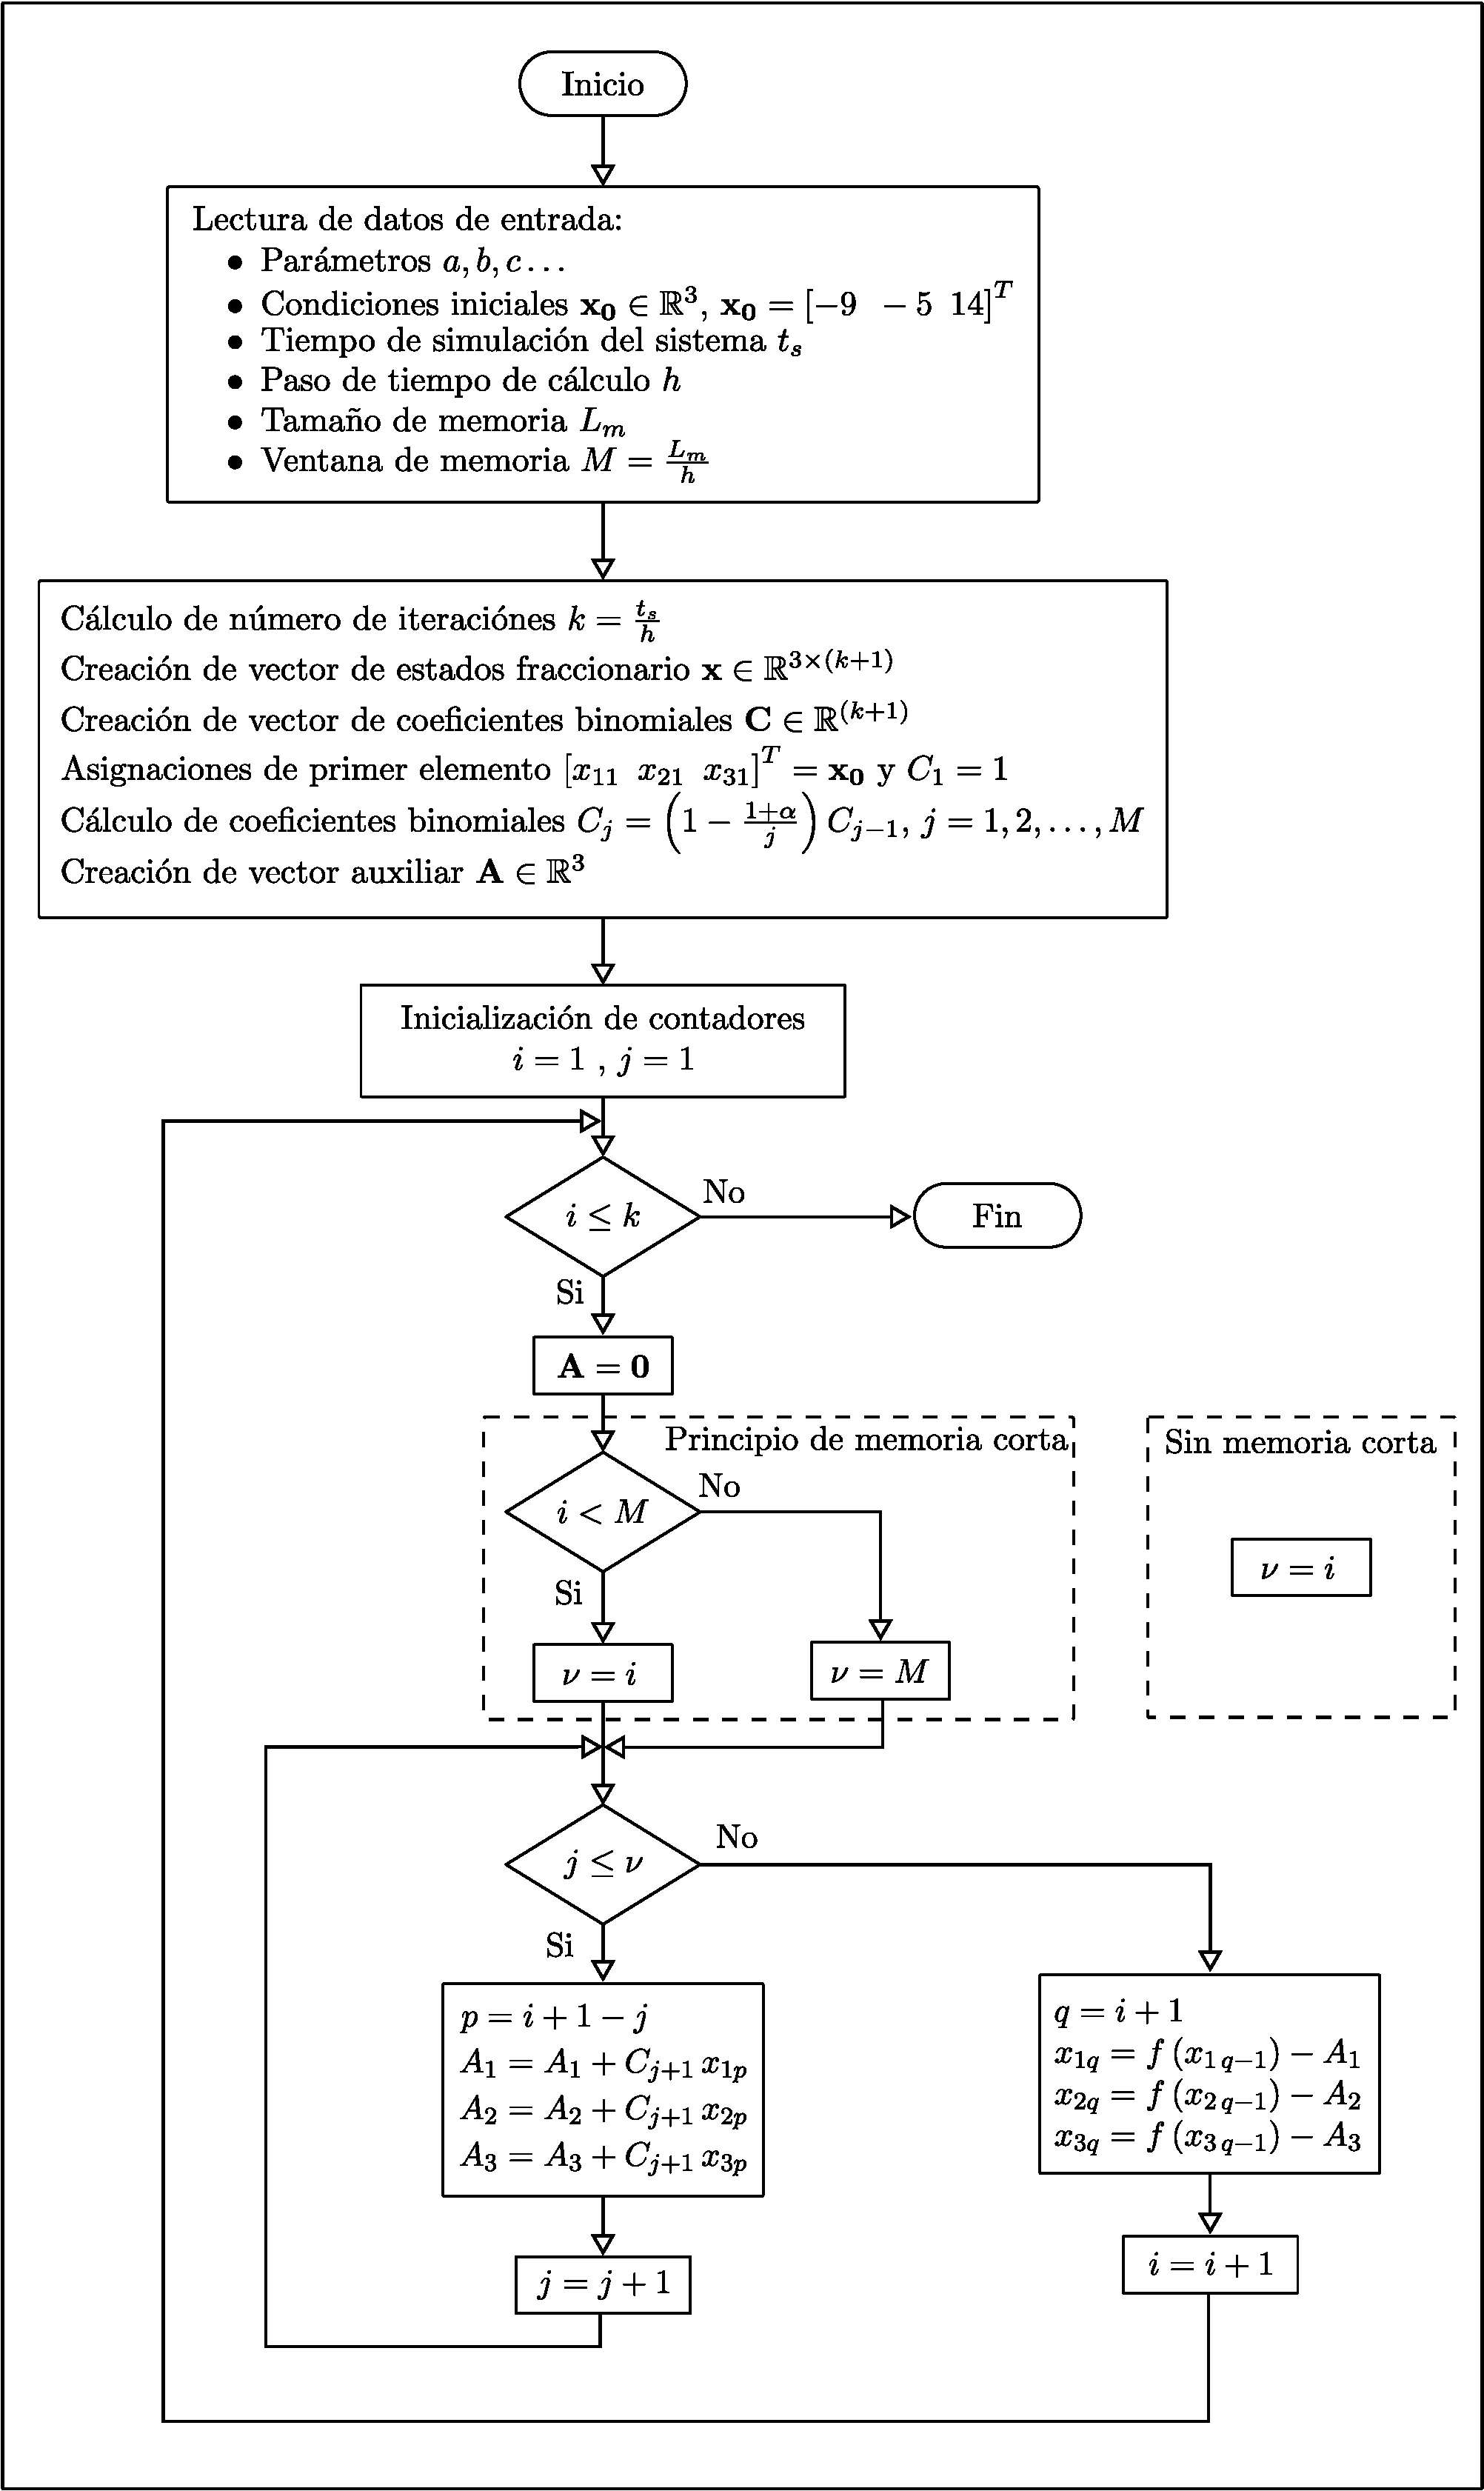
\includegraphics[width = 4cm]{diag_flug_GL.pdf}
			\caption{Diagrama de flujo de método numérico de GL.}
		\end{figure}
	\end{frame}	
%%----------------------------------------------------------------------------------
%%----------------------------------------------------------------------------------
	\begin{frame}
		\frametitle{Fundamentos teóricos}
		\begin{block}{Oscilador SNLF (Funciones No Lineales Saturadas)}
		\justifying
		\begin{equation} 
		\begin{array}{lcl}
		\dot{x_{1}} & = & x_{2} \\
		\dot{x_{2}} & = & x_{3}\\
		\dot{x_{3}} & = & -a x_{1} - b x_{2} -c x_{3} + d_{1} f(x_{1};m)
		\end{array}
		\label{ec:oscilador}
	\end{equation}
		\end{block}
		
		\begin{figure}[hbtp]
			\centering
			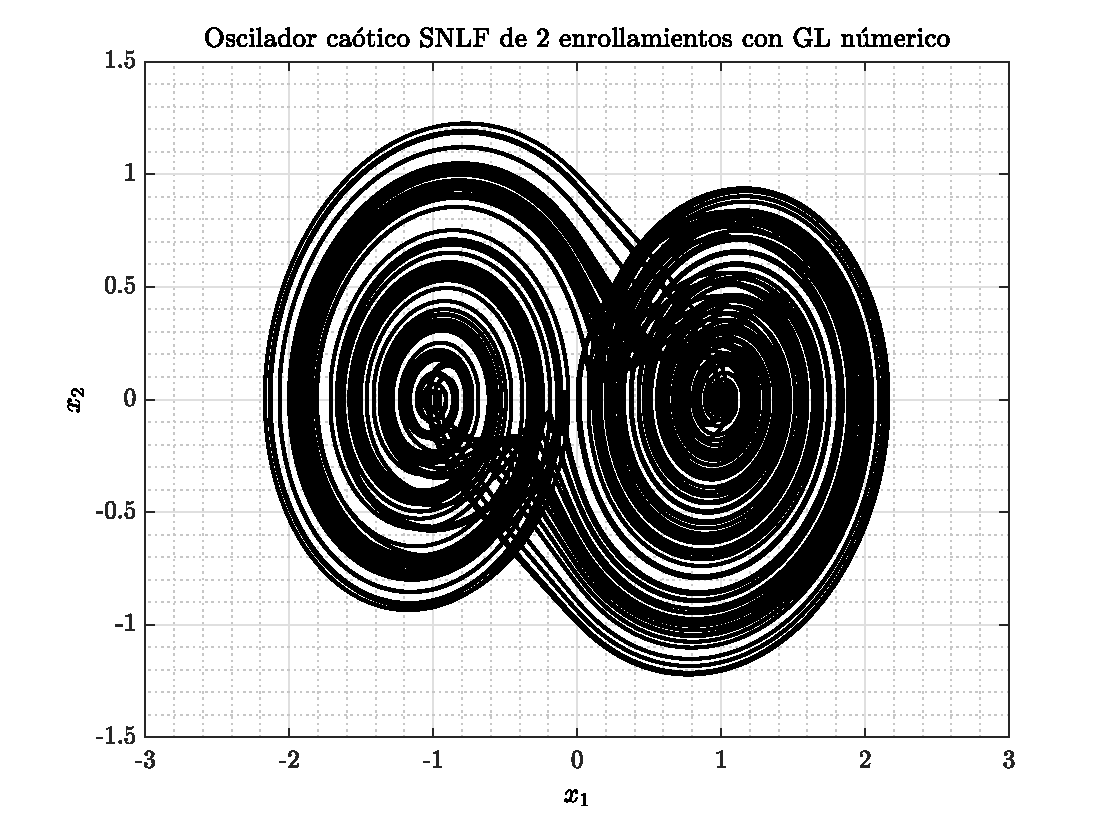
\includegraphics[width = 6cm]{gl_num.pdf}
			\caption{ Simulación de método numérico de GL.}
		\end{figure}
	\end{frame}	
%%----------------------------------------------------------------------------------
%%----------------------------------------------------------------------------------	
	\begin{frame}
		\frametitle{Fundamentos teóricos}
		\begin{block}{Serie de funciones saturadas}
		\justifying
		\begin{equation} 
	f_{0}(x_{1},m)= \left\{ \begin{array}{lcl}
	1 & \text{ si } & x_{1} > m \\
	\frac{x_{1}}{m}& \text{ si } & |x_{1}| \leq m\\
	-1 & \text{ si } & x_{1} < -m
	\end{array}
	\right.
	\label{ec:f0}
\end{equation}


\begin{equation} 
	f_{h}(x_{1},m,h)= \left\{ \begin{array}{lcl}
	2 & \text{ si } & x_{1} > h + m \\
	\frac{x_{1}-h}{m}& \text{ si } & |x_{1} - h| \leq m\\
	0 & \text{ si } & x_{1} < h-m
	\end{array}
	\right.
		\label{ec:fh}
\end{equation}

\begin{equation} 
	f_{-h}(x_{1},m,-h)= \left\{ \begin{array}{lcl}
	0 & \text{ si } & x_{1} > h + m \\
	\frac{x_{1}-h}{m}& \text{ si } & |x_{1} - h| \leq m\\
	-2 & \text{ si } & x_{1} < h-m
	\end{array}
	\right.
		\label{ec:f-h}
\end{equation}
		\begin{equation}
f(x,m) = \sum_{i=0}^{s-2} f_{2i-s+2}(x,m,2i-s+2)
\label{ec:general_serie}
\end{equation}
		\end{block}
	\end{frame}
%%----------------------------------------------------------------------------------
%%----------------------------------------------------------------------------------	
	\begin{frame}
		\frametitle{Fundamentos teóricos}

		
		\begin{figure}[hbtp]
			\centering
			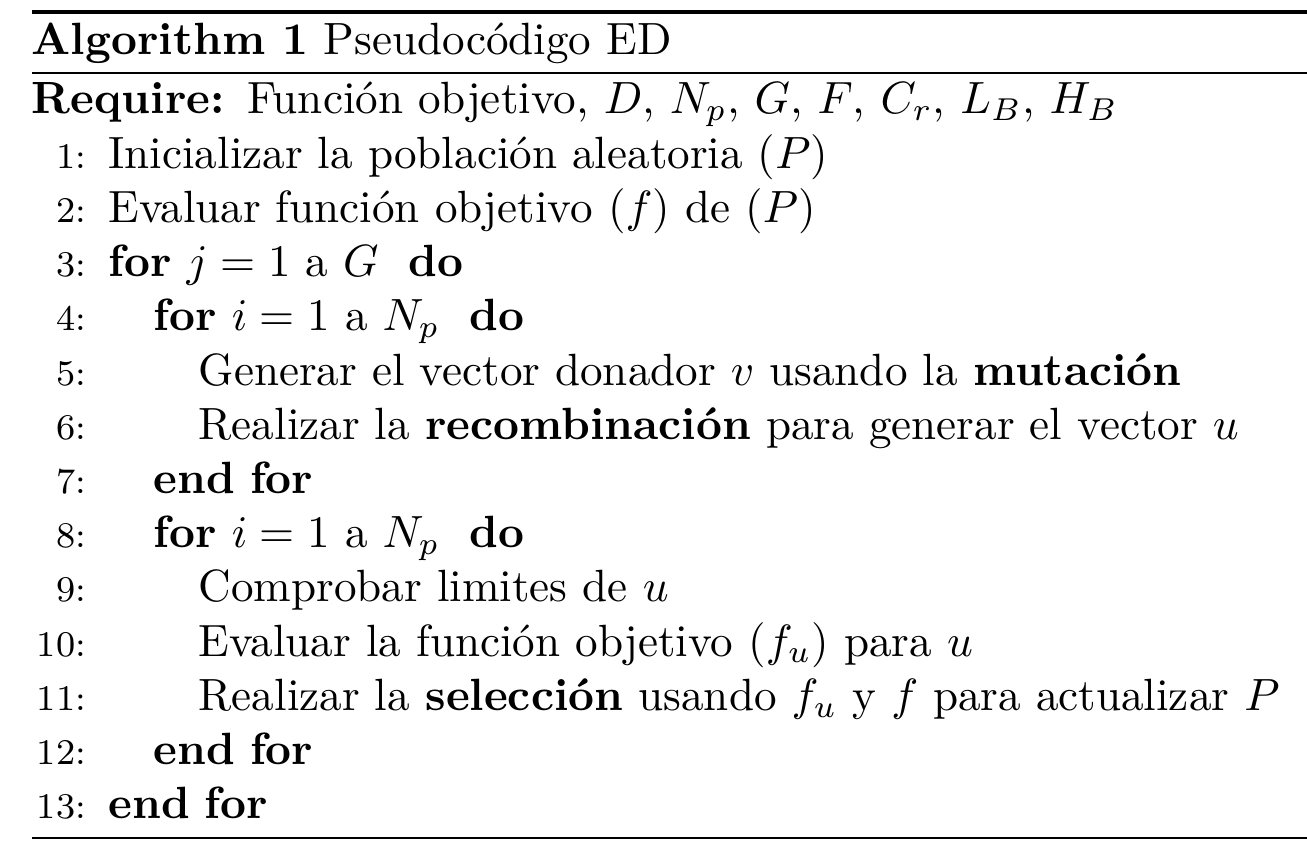
\includegraphics[width = 6cm]{alg1.png}
			\caption{Algoritmo de Evolución Diferencial.}
		\end{figure}
		
	\end{frame}
%%----------------------------------------------------------------------------------
%%----------------------------------------------------------------------------------	
	\begin{frame}
		\frametitle{Fundamentos teóricos}

		
		\begin{figure}[hbtp]
			\centering
			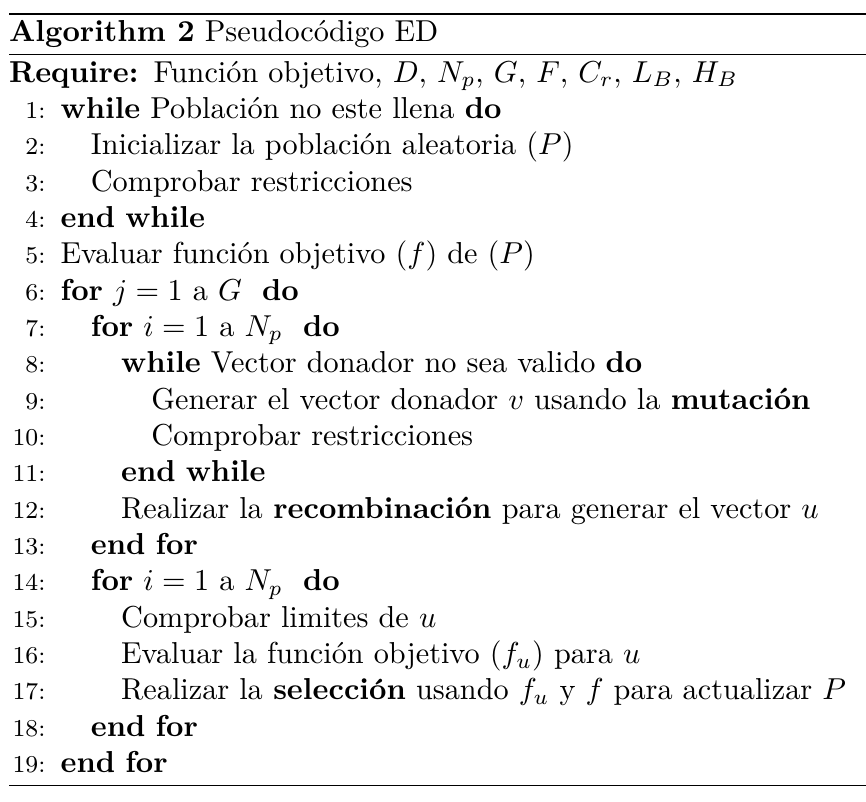
\includegraphics[width = 6cm]{alg2.png}
			\caption{Algoritmo de Evolución Diferencial modificado.}
		\end{figure}
		
	\end{frame}
%%----------------------------------------------------------------------------------
%%----------------------------------------------------------------------------------		

	\section{Resultados}
	
	
	\begin{frame}
		\frametitle{Resultados}

		
		\begin{figure}[hbtp]
			\centering
			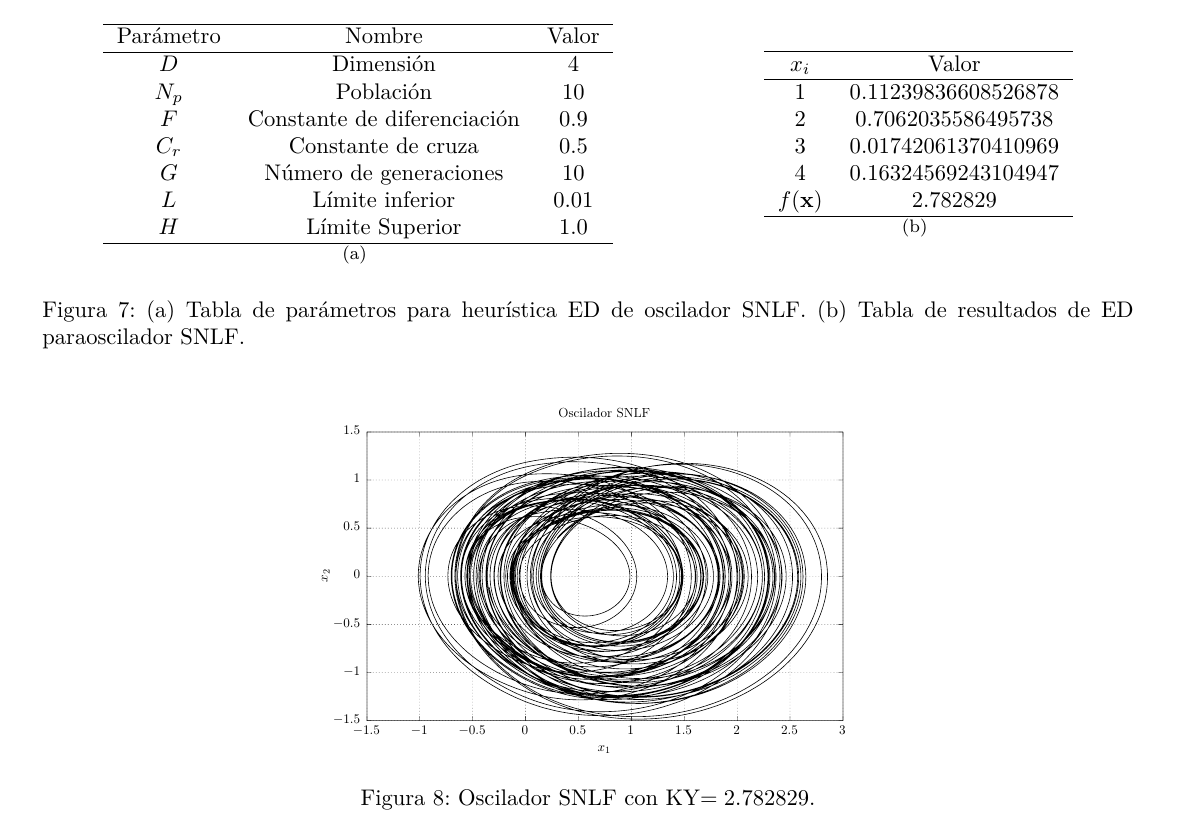
\includegraphics[width = 10cm]{ex1.png}
		\end{figure}
		
	\end{frame}
	
		\begin{frame}
		\frametitle{Resultados}

		
		\begin{figure}[hbtp]
			\centering
			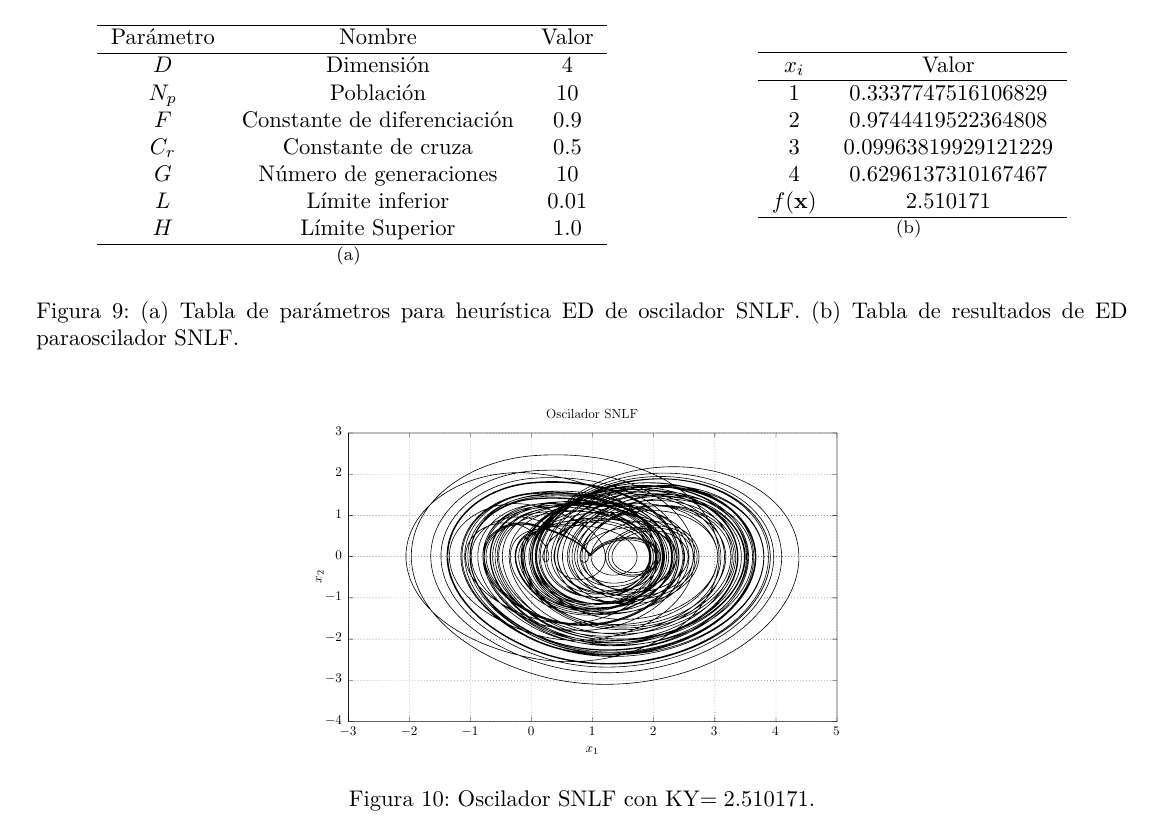
\includegraphics[width = 10cm]{ex2.png}
		\end{figure}
		
	\end{frame}
	
		\begin{frame}
		\frametitle{Resultados}

		
		\begin{figure}[hbtp]
			\centering
			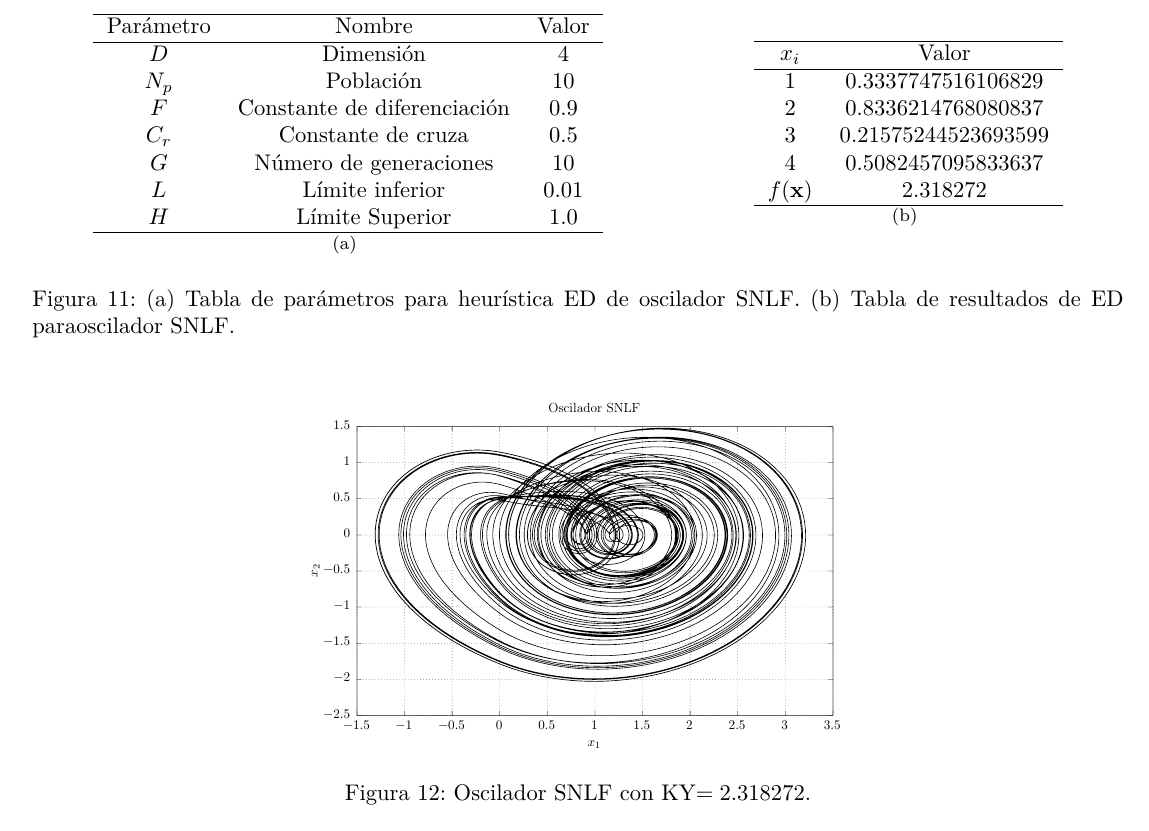
\includegraphics[width = 10cm]{ex3.png}
		\end{figure}
	\end{frame}
	
	
	\begin{frame}
		\frametitle{Resultados}

		
		\begin{figure}[hbtp]
			\centering
			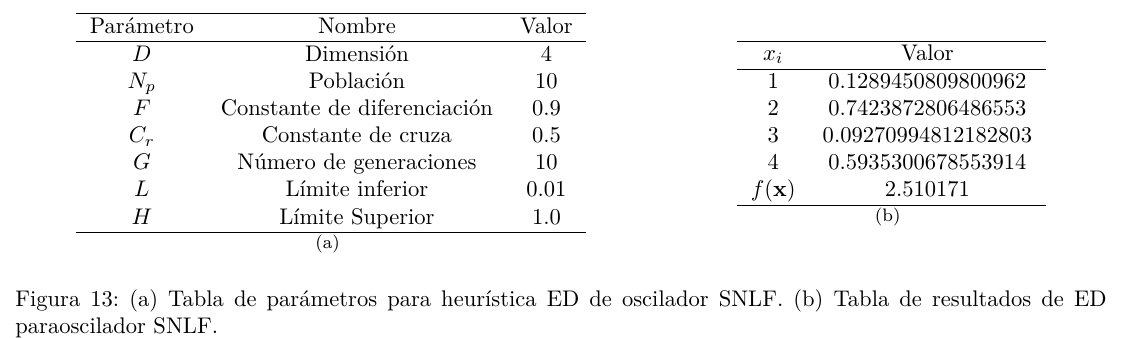
\includegraphics[width = 10cm]{ex4a.png}
			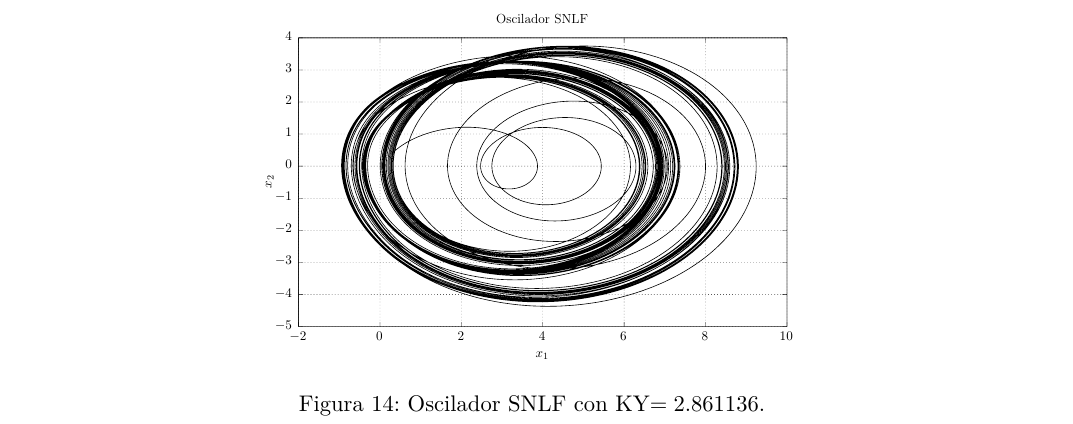
\includegraphics[width = 10cm]{ex4b.png}
		\end{figure}
	\end{frame}


%%----------------------------------------------------------------------------------
%%----------------------------------------------------------------------------------
	\section{Conclusión}
	\begin{frame}
		\frametitle{Conclusión}
		\begin{block}{Conclusiones}
			\begin{itemize}
				\item Se logró aumentar la dimensión KY.
				\item Es necesario tener cuidado con la calibración de lyap\_{}spec de TISEAN. 
				
				\item Las restricciones son muy importantes porque de lo contrario falla lyap\_{}spec.

				\item Trabajo futuro:
					\begin{itemize}
						\item Optimizar agregando el orden fraccionario a la dimensión de la ED.
					\end{itemize}

			\end{itemize}
		\end{block}
	\end{frame}	
	
	
	
	
	
	
	
	
	
	\section{Bibliografía}
	\begin{frame}[t, allowframebreaks]
		\frametitle{Bibliografía}
		\nocite{*}
		\bibliographystyle{ieeetr}
		\bibliography{bibliografia}
	\end{frame}
	
	

\end{document}